
% Graph analysis has been attracting increasing attention in the
% recent years due the ubiquity of networks in the real world. Graphs
% (a.k.a. networks) have been used to denote information in various
% areas including biology (Protein-Protein interaction networks),
% social sciences (friendship networks), and linguistics (word co-occurrence networks) \Omri{Consider adding citations to these examples}\Roni{Yes}. 
% Modeling the interactions between entities as graphs has enabled researchers to understand the various network systems in a systematic manner{\cite{goyal2018graph}}. 
% Hereby MAPF classical problem that is basically a grid with start and goal location of the agents can be represented as a graph - the grid locations are nodes and edges exist only between nodes that are adjacent to each other i.e agents can move between them. \Omri{The definition of classical MAPF problem as a graph will be given in previous sections (BACKGROUND or INTRO I guess), so you can remove this sentence}.
% Recently, the methods based on representing networks/graphs \Omri{I suggest only writing "graphs" in this context and not "networks" to reduce confusion} in vector space, while preserving their properties, have become widely popular \Omri{I am not familiar with the field, but I guess you are referring to graph embeddings. Consider rephrasing this sentence to: "However, training a model directly on graphs suffer from high computational cost, especially for sparse graphs that are common for classical MAPF problems. Recently, graph embedding techniques -- cite papers on graph embeddings -- have shown remarkable success of converting high-dimensional sparse graphs into low-dimensional, dense and continuous vector
% space"}.
% We utilize graph embedding methods to encode the classical MAPF problem.
% Obtaining such an embedding is useful in the tasks such as classification. The embeddings are input as features to a ML model and the parameters are learned based on the training data. This obviates the need for complex classification models which are applied directly on the graph{\cite{goyal2018graph}}. \Omri{This should be specified in the sentences above, where I wrote "However, training a model...". Add the citations there?}

% \subsection{Using Feather model}\vspace{10px}
% \label{scn:Feather}
% % \subsubsection{\textbf{FEATHER Algorithm}}\vspace{10px}


% Rozemberczki et al.~\cite{rozemberczki2020characteristic}, proposed FEATHER, a flexible notion of characteristic functions defined on graph vertices to describe the distribution of vertex features at multiple scales. 
% %, Introduce FEATHER \Omri{Remove last two words and comma since we wrote FEATHER above}. 
% FEATHER is a computationally
% efficient algorithm to calculate a specific variant of these characteristic functions where the probability weights of the characteristic function are defined as the transition probabilities of random walks. Features extracted by this procedure are useful for
% node-level machine learning tasks. Also discuss the pooling of these node representations, resulting in compact descriptors of graphs that can serve as features for graph classification algorithms, another positive property is that FEATHER describes isomorphic graphs with the same representation and exhibits robustness to data corruption. \Omri{I think you should rephrase but I have no good suggestion. If you want we can do it together on a zoom call.}
% we will use this method as part of our MAPFGAS model.


% \begin{figure}[!h]
%     \centering
%     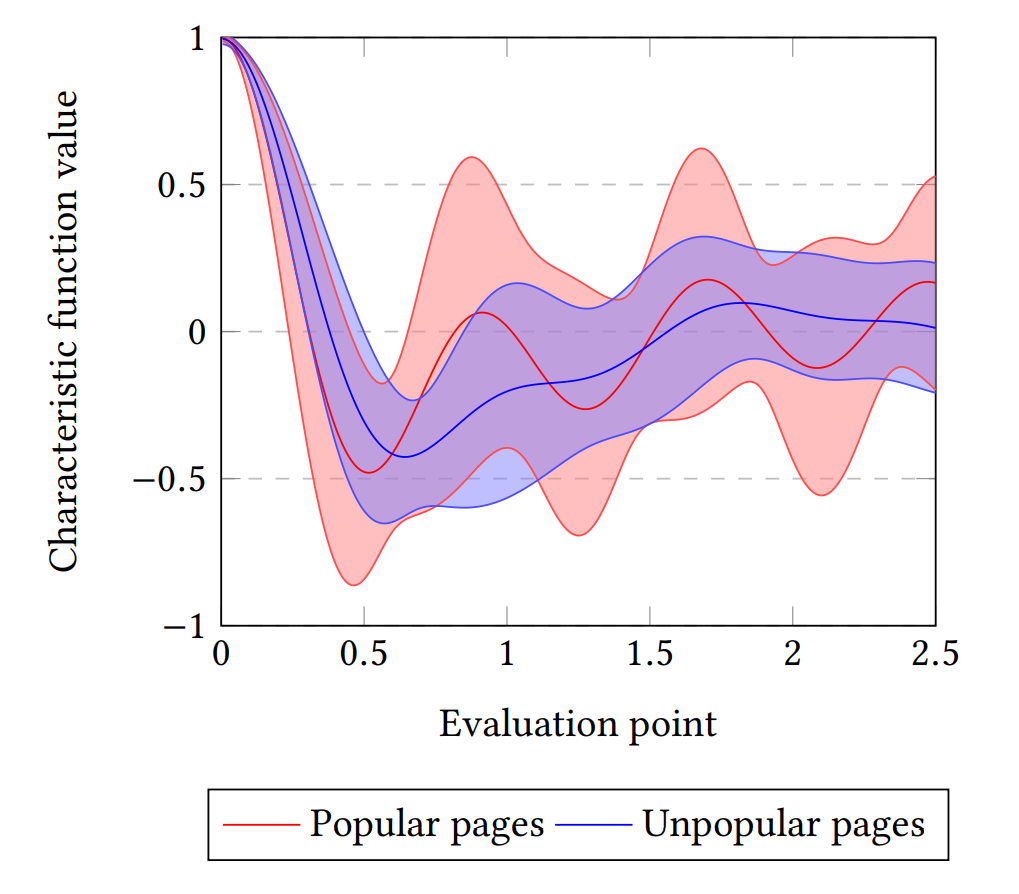
\includegraphics[scale=0.32]{Images/Feather_1.png}
%     \caption{The real part of class dependent mean characteristic functions with standard deviations around the mean for the log transformed degree on the Wikipedia Crocodiles dataset.}
%     % \cite{rozemberczki2020characteristic}
%     \label{fig:Feather}
% \end{figure}

% \textbf{A Conceptual Overview} \Omri{Maybe change to: Method overview} is provided in Figure \ref{fig:Feather}. It shows the distribution of node-level characteristic function values on the Wikipedia Crocodiles web graph \Omri{Is there a citation for this graph?}. In this dataset, nodes are web pages that have two types of labels – popular and unpopular \Omri{Rehprase to: ... nodes are web pages that are labeled as popular or nonpopular}. With log transformed degree centrality as
% the vertex attribute, we conditioned the distributions on the class
% memberships. We plotted the mean of the distribution at each evaluation point with the standard deviation around the mean. One can easily observe that the value of the characteristic function is discriminating with respect to the class membership of nodes {\cite{rozemberczki2020characteristic}}.
% \Roni{Above conceptual overview is probably redundant as it is hard to relate to our problem setting. I'll think about it}

% \subsection{\textbf{Key Points Method Description}} \vspace{10px}
% \subsection{Key Points Method Description} \vspace{10px}
% \label{scn:MAPFGAS design}








% \begin{table*}[tbh!]
% \resizebox{\textwidth}{!}{
% \begin{tabular}{@{}ll|rrr|rrr|rrr|rrr|rrr|rrr|rrr@{}}
% \toprule
%                               & Grid-type & \multicolumn{3}{c}{Empty}                    & \multicolumn{3}{c}{Random}                   & \multicolumn{3}{c}{Warehouse}                 & \multicolumn{3}{c}{Game}                       & \multicolumn{3}{c}{City}                       & \multicolumn{3}{c}{Maze}                       & \multicolumn{3}{c}{Room}                       \\ 
% AS Setup                      & Metric    & Acc           & Cov           & \%Rg         & Acc           & Cov           & \%Rg         & Acc           & Cov           & \%Rg          & Acc           & Cov           & \%Rg           & Acc           & Cov           & \%Rg           & Acc           & Cov           & \%Rg           & Acc           & Cov           & \%Rg           \\
% \midrule
% \multirow{3}{*}{In-Grid}      & KBS       & 0.88          & \textbf{1.00} & 0.9          & \textbf{0.91} & \textbf{1.00} & 3.1          & 0.84          & 0.99          & 7.9           & 0.91          & 0.98          & 19.2           & 0.90          & \textbf{0.99} & 10.1           & 0.85          & 0.98          & 31.9           & \textbf{0.93} & \textbf{1.00} & 0.2            \\
%                               & G2V       & 0.89          & \textbf{1.00} & 0.1          & 0.90          & \textbf{1.00} & 4.1          & 0.84          & 0.99          & 9.4           & 0.91          & 0.98          & 21.0           & 0.89          & \textbf{0.99} & 12.4           & 0.79          & 0.93          & 119.3          & 0.90          & \textbf{1.00} & 2.1            \\
%                               & MAG       & \textbf{0.90} & \textbf{1.00} & \textbf{0.8} & \textbf{0.91} & \textbf{1.00} & \textbf{2.4} & \textbf{0.86} & \textbf{1.00} & \textbf{4.7}  & \textbf{0.92} & \textbf{0.99} & \textbf{18.0}  & \textbf{0.92} & \textbf{0.99} & \textbf{7.1}   & \textbf{0.86} & \textbf{0.99} & \textbf{20.6}  & 0.92          & \textbf{1.00} & \textbf{0.1}   \\
% \midrule
% \multirow{3}{*}{In-Grid-Type} & KBS       & 0.67          & 0.97          & 3.5          & \textbf{0.84} & \textbf{1.00} & 1.4          & 0.64          & 0.94          & 1.4           & 0.77          & \textbf{0.92} & \textbf{1.4}   & 0.58          & 0.81          & 3.1            & 0.40          & \textbf{0.66} & \textbf{8.2}   & 0.63          & 0.91          & 2.9            \\
%                               & G2V       & 0.68          & \textbf{1.00} & \textbf{1.0} & 0.79          & 0.99          & 2.3          & 0.64          & 0.94          & 1.6           & 0.72          & 0.86          & 2.3            & 0.57          & \textbf{0.83} & 3.0            & 0.44          & 0.62          & 9.6            & 0.50          & 0.83          & 5.0            \\
%                               & MAG       & \textbf{0.71} & 0.99          & 1.8          & 0.82          & \textbf{1.00} & \textbf{1.1} & \textbf{0.67} & \textbf{0.96} & \textbf{1.3}  & \textbf{0.78} & \textbf{0.92} & 1.7            & \textbf{0.61} & \textbf{0.83} & \textbf{2.9}   & \textbf{0.50} & \textbf{0.66} & 8.4            & \textbf{0.66} & \textbf{0.94} & \textbf{2.2}   \\
% \midrule
% \multirow{3}{*}{Between-Grid} & KBS       & 0.81          & \textbf{1.00} & 9.5          & \textbf{0.78} & \textbf{1.00} & 7.2          & 0.67          & 0.96          & 32.9          & \textbf{0.74} & 0.88          & 122.0          & 0.53          & \textbf{0.90} & \textbf{136.2} & \textbf{0.56} & \textbf{0.71} & \textbf{398.8} & 0.32          & 0.65          & 855.6          \\
%                               & G2V       & 0.78          & 0.99          & 17.7         & 0.71          & 0.99          & 54.8         & 0.62          & 0.88          & 78.1          & 0.72          & \textbf{0.89} & \textbf{113.1} & 0.53          & 0.86          & 155.6          & 0.45          & 0.64          & 511.4          & 0.43          & 0.75          & 614.5          \\
%                               & MAG       & \textbf{0.82} & \textbf{1.00} & \textbf{2.5} & 0.73          & \textbf{1.00} & \textbf{4.0} & \textbf{0.68} & \textbf{0.98} & \textbf{27.3} & 0.65          & \textbf{0.89} & 122.0          & \textbf{0.58} & 0.88          & 146.3          & 0.47          & 0.66          & 483.6          & \textbf{0.49} & \textbf{0.81} & \textbf{475.0} \\ \bottomrule 
% \end{tabular}
% }
% \label{tab:by-grid-type}
% \caption{Results for all AS setups, grouped by test grid type.}
% \end{table*}



% Please add the following required packages to your document preamble:
% \usepackage{booktabs}
% \usepackage{multirow}



% % Please add the following required packages to your document preamble:
% % \usepackage{booktabs}
% \begin{table}
% \centering
% \begin{tabular}{@{}lrrrr@{}}
% \toprule
% Metric   & \multicolumn{1}{c}{Acc} & \multicolumn{1}{c}{Cov} & \multicolumn{1}{c}{RT} & \multicolumn{1}{c}{\% Rg} \\ \midrule
% KGS      & 0.69                    & 0.93                    & 0.86                   & 78.60                     \\
% G2V      & 0.67                    & 0.92                    & 0.91                   & 91.80                     \\
% MAPFGAS  & \textbf{0.71}                    & \textbf{0.94}                    & \textbf{0.80}                   & \textbf{67.90}                     \\ \midrule
% Oracle   & 1.00                    & 1.00                    & 0.48                   & 0.00                      \\ \midrule
% FG2V+G2V & 0.69                    & 0.93                    & 0.84                   & 75.80                     \\
% KGS+FG2V & 0.70                    & 0.94                    & 0.81                   & 70.50                     \\
% KGS+G2V  & 0.70                    & 0.94                    & 0.82                   & 71.60                     \\
% FG2V     & 0.66                    & 0.91                    & 0.90                   & 87.90                     \\ \bottomrule
% \end{tabular}
% \label{tab:in-grid-type}
% \caption{Results for the In-Grid-Type AS setup.}
% \end{table}





% Our first observation from these results is 


% that some \kaduri\ features are indeed important. 
% However, they are not sufficient, and feature from each family are important and needed. 

% Another observation is that from each feature family there are substantial number of features whose importance is close to zero. 
% This suggests that applying feature selection method based on weights may in our case be effective. 
% \Roni{Ideally, add here results for the feature importance analysis of the other AS setups} \Carmel{do you want similar plots for other setups?}
% even more (the initial Graphs representing each MAPF problem is much bigger) \Roni{Not clear. What do you mean by the MAPF graphs being much bigger - much larger than what?} \Carmel{the Feather graph embedding dim is 500 assume in XGB 50\% of coefs are zero => 250 dimensions from 500 are not important at all for classification so we can cut them...}
% \Roni{Can you extract which of the hand-crafted features were not useful (their actual values)?} \Carmel{yes it in the csv files I sent}
% \Roni{Cosmetics: might be nicer to sort by importance in each feature family. Not important} \Carmel{If we want to compare feature importance between experiments we should not sort, every feature index is it's uniqueness}


% from \fgtv. established by the FullG2V abstraction the next 500 established by the G2V (using Feather model \cite{rozemberczki2020characteristic}), the remaining 20 are the handcrafted features obtained Kaduri's method \cite{kaduri2020algorithm}. we can see an interesting observation, that the handcrafted features are relatively high, also we can see that there are substantial number of features coefficients that are zero or close, thus a feature selection method based on weights can be used to reduce substantially the embeddings dimension even more (the initial Graphs representing each MAPF problem is much bigger) \Roni{Not clear. What do you mean by the MAPF graphs being much bigger - much larger than what?} \Carmel{the Feather graph embedding dim is 500 assume in XGB 50\% of coefs are zero => 250 dimensions from 500 are not important at all for classification so we can cut them...}
% \Roni{Can you extract which of the hand-crafted features were not useful (their actual values)?} \Carmel{yes it in the csv files I sent}
% \Roni{Cosmetics: might be nicer to sort by importance in each feature family. Not important} \Carmel{If we want to compare feature importance between experiments we should not sort, every feature index is it's uniqueness}


% \begin{figure}
%     \centering
%     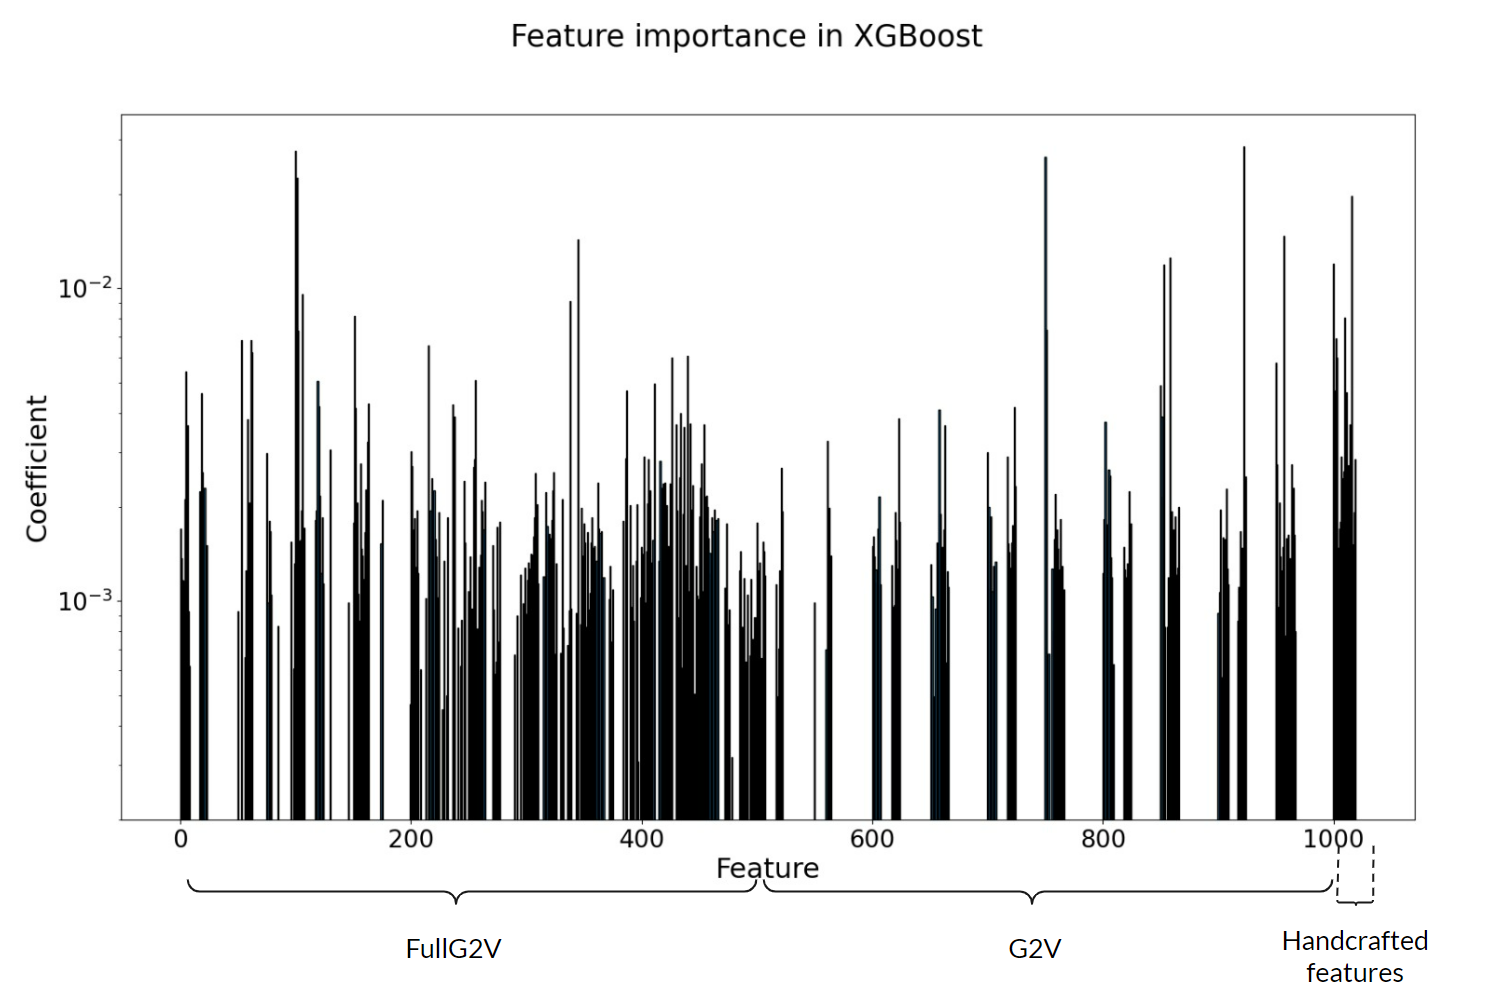
\includegraphics[scale=0.23]{Images/feature_importance_xgb.png}
%     \caption{Features importance for the MAPFGAS abstraction method in the XGBoost classifier.}
%     \label{fig:model_coefs}
% \end{figure}



% Please add the following required packages to your document preamble:
% \usepackage{booktabs}
% \begin{table}
% \begin{tabular}{@{}ll|rrr|r@{}}
% \toprule
% Grid-type & Metric & KBS   & G2V   & MAFGAS \\ \midrule
% City      & Acc    & 0.53  & 0.53  & 0.58   \\
% City      & Cov    & 0.896 & 0.863 & 0.877  \\
% City      & \%Rg   & 136.2 & 155.6 & 146.3  \\
% Empty     & Acc    & 0.81  & 0.78  & 0.82   \\
% Empty     & Cov    & 0.996 & 0.993 & 0.9991 \\
% Empty     & \%Rg   & 9.5   & 17.7  & 2.5    \\
% Game      & Acc    & 0.74  & 0.72  & 0.65   \\
% Game      & Cov    & 0.875 & 0.891 & 0.894  \\
% Game      & \%Rg   & 122.0 & 113.1 & 122.0  \\
% Random    & Acc    & 0.78  & 0.71  & 0.73   \\
% Random    & Cov    & 0.999 & 0.989 & 1      \\
% Random    & \%Rg   & 7.2   & 54.8  & 4.0    \\
% Room      & Acc    & 0.32  & 0.43  & 0.49   \\
% Room      & Cov    & 0.652 & 0.752 & 0.807  \\
% Room      & \%Rg   & 855.6 & 614.5 & 475.0  \\
% Maze      & Acc    & 0.56  & 0.45  & 0.47   \\
% Maze      & Cov    & 0.706 & 0.635 & 0.655  \\
% Maze      & \%Rg   & 398.8 & 511.4 & 483.6  \\
% Warehouse & Acc    & 0.67  & 0.62  & 0.68   \\
% Warehouse & Cov    & 0.964 & 0.882 & 0.975  \\
% Warehouse & \%Rg   & 32.9  & 78.1  & 27.3   \\ \bottomrule
% \end{tabular}
% \end{table}


% % Please add the following required packages to your document preamble:
% % \usepackage{booktabs}
% % \usepackage{multirow}
% \begin{table}
% \begin{tabular}{@{}ll|rrr|r@{}}
% \toprule
% Grid-type                  & Metric & KBS   & G2V   & MAFGAS \\ \midrule
% \multirow{3}{*}{City}      & Acc    & 0.53  & 0.53  & 0.58   \\
%                            & Cov    & 0.896 & 0.863 & 0.877  \\
%                            & \%Rg   & 136.2 & 155.6 & 146.3  \\ \midrule
% \multirow{3}{*}{Empty}     & Acc    & 0.81  & 0.78  & 0.82   \\
%                            & Cov    & 0.996 & 0.993 & 0.9991 \\
%                            & \%Rg   & 9.5   & 17.7  & 2.5    \\\midrule
% \multirow{3}{*}{Game}      & Acc    & 0.74  & 0.72  & 0.65   \\
%                            & Cov    & 0.875 & 0.891 & 0.894  \\
%                            & \%Rg   & 122.0 & 113.1 & 122.0  \\\midrule
% \multirow{3}{*}{Random}    & Acc    & 0.78  & 0.71  & 0.73   \\
%                            & Cov    & 0.999 & 0.989 & 1      \\
%                            & \%Rg   & 7.2   & 54.8  & 4.0    \\\midrule
% \multirow{3}{*}{Room}      & Acc    & 0.32  & 0.43  & 0.49   \\
%                            & Cov    & 0.652 & 0.752 & 0.807  \\
%                            & \%Rg   & 855.6 & 614.5 & 475.0  \\\midrule
% \multirow{3}{*}{Maze}      & Acc    & 0.56  & 0.45  & 0.47   \\
%                            & Cov    & 0.706 & 0.635 & 0.655  \\
%                            & \%Rg   & 398.8 & 511.4 & 483.6  \\\midrule
% \multirow{3}{*}{Warehouse} & Acc    & 0.67  & 0.62  & 0.68   \\
%                            & Cov    & 0.964 & 0.882 & 0.975  \\
%                            & \%Rg   & 32.9  & 78.1  & 27.3   \\ \bottomrule 
% \end{tabular}
% \end{table}


% Please add the following required packages to your document preamble:
% \usepackage{booktabs}
% \usepackage{multirow}
% \begin{table}
% \centering
% \begin{tabular}{@{}ll|rrr|r@{}}
% \toprule
% Grid-type                  & Metric & KBS    & G2V    & MAFGAS & Oracle \\ \midrule
% \multirow{3}{*}{City}      & Acc    & 0.53   & 0.53   & 0.58   & 1.00   \\
%                            & Cov    & 0.90   & 0.86   & 0.88   & 1.00   \\
%                            & RT     & 13,218 & 14,308 & 13,784 & 5,597  \\ \midrule
% \multirow{3}{*}{Empty}     & Acc    & 0.81   & 0.78   & 0.82   & 1.00   \\
%                            & Cov    & 1.00   & 0.99   & 1.00   & 1.00   \\
%                            & RT     & 3,372  & 3,626  & 3,157  & 3,080  \\\midrule
% \multirow{3}{*}{Game}      & Acc    & 0.74   & 0.72   & 0.65   & 1.00   \\
%                            & Cov    & 0.88   & 0.89   & 0.89   & 1.00   \\
%                            & RT     & 16,187 & 15,537 & 16,187 & 7,292  \\\midrule
% \multirow{3}{*}{Random}    & Acc    & 0.78   & 0.71   & 0.73   & 1.00   \\
%                            & Cov    & 1.00   & 0.99   & 1.00   & 1.00   \\
%                            & RT     & 1,717  & 2,478  & 1,665  & 1,601  \\\midrule
% \multirow{3}{*}{Room}      & Acc    & 0.32   & 0.43   & 0.49   & 1.00   \\
%                            & Cov    & 0.65   & 0.75   & 0.81   & 1.00   \\
%                            & RT     & 6,172  & 4,615  & 3,714  & 646    \\\midrule
% \multirow{3}{*}{Maze}      & Acc    & 0.56   & 0.45   & 0.47   & 1.00   \\
%                            & Cov    & 0.71   & 0.64   & 0.66   & 1.00   \\
%                            & RT     & 4,300  & 5,270  & 5,031  & 862    \\\midrule
% \multirow{3}{*}{Warehouse} & Acc    & 0.67   & 0.62   & 0.68   & 1.00   \\
%                            & Cov    & 0.96   & 0.88   & 0.98   & 1.00   \\
%                            & RT     & 25,813 & 34,584 & 24,718 & 19,416 \\ \bottomrule 
% \end{tabular}
% \end{table}

% Please add the following required packages to your document preamble:
% \usepackage{booktabs}
% \begin{table}[]
% \begin{tabular}{@{}lcccccccc@{}}
% Metric & KGS              & G2V              & MAPFGAS          & Oracle         & FG2V+G2V         & KGS+FG2V         & KGS+G2V          & FG2V             \\
% Acc    & (0.64,0.69,0.75) & (0.61,0.67,0.73) & (0.64,0.71,0.77) & (1,1,1)        & (0.63,0.69,0.74) & (0.65,0.7,0.75)  & (0.65,0.7,0.76)  & (0.58,0.66,0.72) \\
% Cov    & (0.9,0.93,0.95)  & (0.9,0.92,0.94)  & (0.91,0.94,0.95) & (1,1,1)        & (0.9,0.93,0.94)  & (0.91,0.94,0.95) & (0.92,0.94,0.95) & (0.88,0.91,0.95) \\
% RT     & (13029,1,24759)  & (16070,1,24681)  & (12188,1,23769)  & (6878,0,14081) & (13159,1,24922)  & (13027,1,23550)  & (12628,1,23317)  & (13861,1,26696)  \\
% \% Rg  & 78.60            & 91.80            & 67.90            & 0.00           & 75.80            & 70.50            & 71.60            & 87.90           
% \end{tabular}
% \end{table}

% results show similar to those in Table performance in most cases




% describes experiments done "in grid split" setups. In the first experiment a random split was performed on all MAPF problems, while on every other experiment a random split was performed on all MAPF problems that belongs to specific grid type - for example the second row where scope is 'city', the dataset is combined only from all MAPF problems that have a city map.

% we can observe that combining both Graph abstractions G2V and FullG2v with handcrafted features achieved overall similar to the best results in all metrics.

% \begin{table*}[!h]
% % \begin{table}[!h]
%     \centering
% \begin{tabular}{ |c|c||c|c|c||c|c|c|c||c| }
% \hline
%     & &  \multicolumn{8}{|c|}{Topological 'MAPF Problem' Abstraction Method} \\ 
%  \hline
%     scope & metric & hand & G-short & G-full &  hand-full & hand-short & full-short & triple & oracle\\ 
%  \hline
%  & Accuracy  & 0.83 & 0.81 & 0.84 & \textbf{0.85} & 0.84 & 0.84 & \textbf{0.85} & 1.0\\ 
%  all$_{random}$ & Coverage & 0.979 & 0.968 & 0.981 & \textbf{0.986} & 0.982 & 0.981 & \textbf{0.986} & 1.0\\ 
%  & Run-time & 9803 & 10513 & 9527 & \textbf{9150} & 9497 & 9480 & 9180 & 7785\\
%  \hline
%   & Accuracy  & 0.90 & 0.89 & 0.89 & \textbf{0.92} & \textbf{0.92} & 0.91 & \textbf{0.92} & 1.0\\ 
% city & Coverage & 0.992 & 0.986 & 0.989 & \textbf{0.994} & 0.993 & 0.991 & 0.993 & 1.0\\ 
% & Run-time & 1226 & 1252 & 1237 & \textbf{1189} & 1190 & 1216 & 1193 & 1113.7\\ 
%  \hline 
%  & Accuracy  & 0.88 & 0.89 & 0.88 & 0.89 & 0.89 & 0.89 & \textbf{0.90} & 1.0\\ 
%  empty & Coverage & 1.0 & 1.0 & 1.0 & 1.0 & 1.0 & 1.0 & 1.0 & 1.0\\ 
%  & Run-time & 662.1 & \textbf{657} & 665.1 & 661.8 & \textbf{657} & 661.5 & 661.6 & 656.18\\ 
%  \hline
%  & Accuracy  & 0.91 & 0.91 & \textbf{0.92} & \textbf{0.92} & 0.91 & \textbf{0.92} & \textbf{0.92} & 1.0\\ 
% game & Coverage & 0.984 & 0.981 & 0.989 & \textbf{0.990} & 0.984 & 0.988 & 0.985 & 1.0\\ 
% & Run-time & 1718 & 1743 & \textbf{1647} & \textbf{1647} & 1715 & 1675 & 1700 & 1440.7\\ 
%  \hline 
%  & Accuracy  & 0.91 & 0.90 & 0.91 & 0.91 & 0.91 & 0.91 & 0.91 & 1.0\\ 
%  random & Coverage & 0.999 & 0.999 & 1.0 & 1.0 & 1.0 & 0.999 & 1.0 & 1.0\\ 
%  & Run-time & 327.3 & 330.4 & 319.2 & \textbf{318.3} & 318.7 & 330.3 & 325.2 & 317.47\\ 
%  \hline 
%  & Accuracy  & \textbf{0.93} & 0.90 & 0.92 & 0.92 & 0.92 & 0.91 & 0.92 & 1.0\\ 
%  room & Coverage & 1.0 & 1.0 & 1.0 & 1.0 & 1.0 & 1.0 & 1.0 & 1.0\\ 
%  & Run-time & 128.79 & 131.17 & 131.27 & \textbf{128.6} & \textbf{128.6} & 129.37 & \textbf{128.6} & 128.51\\ 
%  \hline 
%  & Accuracy  & 0.85 & 0.79 & 0.84 & \textbf{0.87} & \textbf{0.87} & 0.86 & 0.86 & 1.0\\ 
%  maze & Coverage & 0.983 & 0.925 & 0.979 & 0.988 & 0.986 & 0.979 & \textbf{0.988} & 1.0\\ 
%  & Run-time & 205.36 & 341.37 & 209.1 & \textbf{185.66} & 188.6 & 208.2 & 187.78 & 155.65\\ 
%  \hline
% & Accuracy  & 0.84 & 0.84 & 0.84 &  \textbf{0.86} & 0.85 &  \textbf{0.86} & \textbf{0.86} & 1.0\\ 
% warehouse & Coverage & 0.991 & 0.989 & 0.990 & \textbf{0.995} & 0.993 & 0.994 & \textbf{0.995} & 1.0\\ 
% & Run-time & 4077 & 4131 & 4077 & 3983 & 4027 & 3993 & \textbf{3955} & 3777\\ 
%  \hline 
% \hline
% & Accuracy  & 0.881 & 0.866 & 0.88 & \textbf{\textcolor{red}{0.893}} &  0.889 & 0.888 & \textbf{\textcolor{red}{0.893}} & 1.0\\ 
% \textbf{AVG$_{single}$} & Coverage & 0.991 & 0.981 & 0.991  & \textbf{\textcolor{red}{0.994}} & 0.992 & 0.991 & 0.993 & 1.0\\ 
% % & Run-time & 2268 & 2387 & 2227 & \textbf{\textcolor{red}{2157}} & 2215 & 2212 & 2166 & 1922 \\ 
% & Run-time & 0.4115 & 0.4534 & 0.4086 & \textbf{\textcolor{red}{0.3948}} & 0.4015 & 0.4060 & 0.3974 & 0.3611 \\ 
%  \hline
%  \%$_{avg}$ $>$ oracle & Run-time & 12.4 & 25.4 & 11.8 & \textbf{\textcolor{red}{8.1}} & 9.5 & 11.5 & 9.0 & 0 \\ 
%  \hline
% \end{tabular}
%     \caption{In grid splits results. (Runtime in minutes)\Roni{Please have the results with the same number of decimal points. No need to have more than 2 digits after the decimal point. Additional digits are only confusing and do not really mean anything in our context} \Carmel{In Coverage they actually use 4 digits after dot for example MAPFASTER COV = 96.84\% = 0.9684}\Roni{But such differences in results are really meaningless in our context. Please remove these digits.} \Carmel{reduced to 3 digits in the COV as agreed } }
%     \label{tab:in_grid_test}
% \end{table*}


% % \begin{table}[!h]
% %     \centering
% % \begin{tabular}{ |c|c||c|c|c|c| }
% % \hline
% %      & &  \multicolumn{4}{|c|}{Method} \\ 
% %  \hline
% %   scope & metric & Kaduri  & Graphs & mixed & oracle     \\ 
% % \hline
% %  & acc  &  0.83 & 0.83 & \textbf{0.85} & 1.0 \\ 
% %  all & cov & 0.976 & 0.977 & \textbf{0.984} & 1.0\\ 
% %  & RT & 9913 & 9756 & \textbf{9295} & 7785 \\ 
% %  \hline
% %  \hline
% %  & acc  & 0.89 & 0.88 & \textbf{0.90} & 1.0\\ 
% %  city & cov & 0.985 & 0.986 & \textbf{0.989} & 1.0\\ 
% %  & RT & 1294 & 1272 & \textbf{1241}  & 1114\\ 
% %  \hline
% %  \hline
% %        & acc  & 0.88 & 0.88 & \textbf{0.89} & 1.0\\ 
% %  empty & cov & \textbf{0.9996} & \textbf{0.9996} & \textbf{0.9996} & 1.0\\ 
% %        & RT & 662 & 665.1 & \textbf{661.8} & 656\\ 
% %  \hline
% %   \hline
% %  & acc  &  0.91 & \textbf{0.92} & \textbf{0.92} & 1.0\\ 
% %  game & cov & 0.984 & 0.989 & \textbf{0.990} & 1.0\\ 
% %  & RT & 1718 & \textbf{1645} & \textbf{1647} & 1440\\ 
% %  \hline
% %   \hline
% %  & acc  & \textbf{0.91} & \textbf{0.91} & \textbf{0.91} & 1.0\\ 
% %  random & cov & 0.999 & 0.999 & \textbf{1.0} & 1.0 \\ 
% %  & RT & 325.1 & 322.7 & \textbf{321.2} & 317.4\\ 
% %  \hline
% %   \hline
% %  & acc  &  \textbf{0.92} & 0.91 & \textbf{0.92} & 1.0\\ 
% %  room & cov & \textbf{1.0} & 0.999 & \textbf{1.0} & 1.0\\ 
% %  & RT & 128.75 & 133.6 & \textbf{128.59} & 128.5\\ 
% %  \hline
% %   \hline
% %  & acc  & 0.85 & 0.85 & \textbf{0.86} & 1.0\\ 
% %  maze & cov & 0.980 & 0.975 & \textbf{0.983} & 1.0\\ 
% %  & RT & 201.2 & 213.3 & \textbf{195.6} & 155.6\\ 
% %  \hline
% %   \hline
% %  & acc  &  0.86 & 0.85 & \textbf{0.87} & 1.0\\ 
% %  warehouse & cov & 0.993 & 0.992 & \textbf{0.996} & 1.0\\ 
% %  & RT & 3993 & 4011 & \textbf{3930} & 3777\\ 
% %  \hline
% % \end{tabular}
% %     \caption{In grid splits results}
% %     \label{tab:in_grid_test}
% % \end{table}

% \subsubsection{In Grid Type Split}\vspace{10px}
% \label{result:clf_perf}
% % The test set was sub-sampled by using a constant step size of 10 (and not 1), due to long time to transform into shapelets based features (anomaly ratio is same as in original WADI test-set).
% % Figure \ref{fig:clf_scores} represents the F1 score achieved by classifiers within all experimental configurations.
% Table \ref{tab:within_grid_type} describes accuracies, coverage, RT achieved by different MAPF problem abstraction methods at their best hyper parameters configurations.
% 5 different Train test splits where performed, each has different combination of train-test map split.
% % results with the following maps in test-set: 'empty-32-32', 'random-32-32-20', 'Berlin\_1\_256', 'warehouse-20-40-10-2-1', 'lt\_gallowstemplar\_n', 'maze-128-128-10', 'ht\_mansion\_n', 'room-32-32-4'.
% Overall the best results achieved by the combined abstraction method which uses both Graph abstractions G2V and FullG2v along with handcrafted features proposed by Kaduri \cite{kaduri2020algorithm}. A very interesting trend can be observed between the difficulty of tested MAPF problems which represented by the oracle run-time (we can assume more complex MAPF problems takes longer time for algorithms to solve) to the coverage and RT improvement achieved by the mixed MAPFGAS over Kaduri's method.





% \begin{table*}[!h]
% % \begin{table}[!h]
%     \centering
% \begin{tabular}{ |c|c||c|c|c||c|c|c|c||c| }
% \hline
%     & &  \multicolumn{8}{|c|}{Topological 'MAPF Problem' Abstraction Method} \\ 
%  \hline
%     test & metric & hand & G-short & G-full &  hand-full & hand-short & full-short & triple & oracle\\ 
%  \hline
%  & Accuracy  & 0.67 & 0.63 & 0.66 & \textbf{0.68} & \textbf{0.68} & 0.66 & 0\textbf{.68} & 1.0\\ 
%  1 & Coverage & 0.944 & 0.895 & 0.931 & 0.945 & 0.949 & 0.942 & \textbf{0.954} & 1.0\\ 
%  & Run-time & 13029 & 17037 & 13861 & 13027 & 12628 & 13159 & \textbf{12188} & 6878\\ 
%  \hline % {19072}
%  & Accuracy  & 0.75 & 0.73 & 0.72 & 0.75 & 0.76 & 0.74 & \textbf{0.77} & 1.0\\ 
%  2 & Coverage & 0.949 & 0.931 & 0.948 & \textbf{0.953} & 0.952 & 0.937 & 0.952 & 1.0\\ 
%  & Run-time & 14186 & 16070 & 14458 & \textbf{13735} & 13984 & 15348 & 13931 & 9771\\ 
%  \hline % {21493}
%  & Accuracy  & 0.64 & 0.61 & 0.58 & \textbf{0.65} & \textbf{0.65} & 0.63 & 0.64 & 1.0\\ 
%  3 & Coverage & 0.900 & 0.900 & 0.879 & 0.911 & \textbf{0.916} & 0.899 & 0.913 & 1.0\\ 
%  & Run-time & 24759 & 24681 & 26696 & 23550 & \textbf{23317} & 24922 & 23769 & 12663\\ 
%  \hline % {22042}
%  & Accuracy  & 0.67 & 0.66 & 0.63 & \textbf{0.69} & \textbf{0.69} & \textbf{0.69} & \textbf{0.69} & 1.0\\ 
%  4 & Coverage & 0.901 & 0.915 & 0.887 & 0.937 & 0.924 & 0.934 & \textbf{0.942} & 1.0\\ 
%  & Run-time & 24494 & 23804 & 25752 & 21130 & 22635 & 22005 & \textbf{21127} & 14081\\ 
%  \hline % {22856}
% & Accuracy  & 0.74 & 0.71 & 0.72 & 0.74 & 0.74 & 0.74 & \textbf{0.75} & 1.0\\ 
% 5 & Coverage & 0.932 & 0.939 & 0.924 & 0.935 & 0.934 & \textbf{0.942} & 0.939 & 1.0\\ 
% & Run-time & 18587 & 17991 & 19282 & 18358 & 18349 & \textbf{17480} & 17909 & 9831\\ 
%  \hline % {24823}
% \hline
% & Accuracy  & 0.694 & 0.668 & 0.662 & 0.702 &  0.704 & 0.692 & \textbf{\textcolor{red}{0.706}} & 1.0\\ 
% \textbf{AVG$_{single}$} & Coverage & 0.925 & 0.916 & 0.9138  & 0.936 & 0.935 & 0.931 & \textbf{\textcolor{red}{0.94}} & 1.0\\ 
% % & Run-time & 19011 & 19916  & 20009 & 17960 & 18182 & 18583 & \textbf{\textcolor{red}{17785}} & 10633 \\ 
% & Run-time & 0.8574 & 0.9054 & 0.9028 & 0.8109 & 0.8200 & 0.8403 & \textbf{\textcolor{red}{0.8023}} & 0.4804 \\ 
%  \hline
%  \%$_{avg}$ $>$ oracle & Run-time & 78.6 & 91.8 & 87.9 & 70.5 & 71.6 & 75.8 & \textbf{\textcolor{red}{67.9}} & 0 \\ 
%  \hline
% \end{tabular}
%     \caption{In Grid type split results.}
%     \label{tab:within_grid_type}
% \end{table*}


% % \begin{table}[!h]
% %     \centering
% % \begin{tabular}{ |c|c||c|c|c|c| }
% % \hline
% %     & &  \multicolumn{4}{|c|}{Method} \\ 
% %  \hline
% %     test & metric & Kaduri  & Graphs & combined & oracle    \\ 
% %  \hline
% %  & Accuracy  & 0.68 & 0.66 & \textbf{0.69} & 1.0\\ 
% %  1 & Coverage & \textbf{0.950} & 0.927 & 0.944 & 1.0\\ 
% %  & Run-time & \textbf{12422} & 14189 & 13063 & 6878\\ 
% %  \hline
% %  \hline
% %  & Accuracy  & 0.75 & 0.72 & \textbf{0.76} & 1.0\\ 
% %  2 & Coverage & 0.950 & 0.946 & \textbf{0.954} & 1.0\\ 
% %  & Run-time & 14016 & 14529 & \textbf{13624} & 9771\\ 
% %  \hline
% %   \hline
% %  & Accuracy  & \textbf{0.63} & 0.58 & \textbf{0.63} & 1.0\\ 
% %  3 & Coverage & 0.905 & 0.866 & \textbf{0.918} & 1.0\\ 
% %  & Run-time & 24486 & 27692 & \textbf{23281} & 12663\\ 
% %  \hline
% %    \hline
% %  & Accuracy  & \textbf{0.67} & 0.65 & \textbf{0.67} & 1.0\\ 
% %  4 & Coverage & 0.889 & 0.900 & \textbf{0.926} & 1.0\\ 
% %  & Run-time & 25698 & 24393 & \textbf{22338} & 14081\\ 
% %  \hline
% % \end{tabular}
% %     \caption{In Grid type split results}\roni{Hard to get an overview from the 4 rows. Perhaps we want an average.}
% %     \label{tab:within_grid_type}
% % \end{table}

% \Carmel{I think its better to remove the confusion matrix, nobody show this and its not that interesting??}\Roni{Removed}
% Table \ref{tab:best_xgb_report} describe results achieved by the combined abstraction method for test number '4', \Roni{What is test '4'?} \Carmel{its just one of the 5 splits, i think we should remove this table and description also, the reason I put it initially is to show the spread of the correct classifications between all solver..} we can see classification scores along all the labels which are the different search algorithms:

% \begin{table}[!h]
%     \centering
% \begin{tabular}{ |c c c c c| }
% \hline
%  & precision & recall  & f1 score  & support \\ 
%  \hline
%  icts & 0.25    &  0.01  & 0.02    &   1557 \\    
%  epea &  0.22   &   0.10 &     0.14 &      2771 \\  
%   sat & 0.00    &  0.00 &     0.00   &     45 \\    
%  cbsh-c & 0.71      & 0.81   &   0.75  &    8662 \\ 
%   lazycbs & 0.69    &  0.81 &   0.75 &      9821 \\    
%  \hline
% \end{tabular}
%     \caption{classification report of best 'combined' model}
%     \label{tab:best_xgb_report}
% \end{table}

% Next is the corresponding confusion matrix:

% $
% \begin{bmatrix} 
% 19  & 233  &  0 &  555  &  750  \\
% 27 & 277 &   0 & 1052 &  1415  \\
% 0 &  1 &   0 &  1  &  43  \\
% 27 & 241 &   16 & 6995 & 1383  \\
% 3 &  504  &  3 & 1314 & 7997 \\
% \end{bmatrix}
% $








% % XGBoost's hyper parameters are: min\_child\_weight = 2 ; gamma = 1.2 ; subsample = 1.0 ; colsample\_bytree = 0.5 ; max\_depth = 6 ; earning\_rate = 5e-05 ;  n\_estimators = 600

% \subsubsection{Between Grid Type Split}\vspace{10px}
% \label{result:between_perf}
% Table \ref{tab:between_grid_test} describes experiments performed at "between grid type split" setups. Each row represents an experiment that shows the tested grid type was used, implicitly all other grid types where in train-set.

% We focus on the coverage and run-time metrics, as the accuracy metric is naturally much lower in such difficult split setups and less important than the other time based metrics.
% combining both Graph abstractions G2V and FullG2v with handcrafted features achieved overall best results. \Carmel{remove next probably}
% We can observe that all "between grid type" split setups except one (when 'maze' in test set) have resulted in higher score either by graph standalone abstraction or by the combined abstraction methods.

% \begin{table*}[!h]
% % \begin{table}[!h]
%     \centering
% \begin{tabular}{ |c|c||c|c|c||c|c|c|c||c| }
% \hline
%     & &  \multicolumn{8}{|c|}{Topological 'MAPF Problem' Abstraction Method} \\ 
%  \hline
%     tested & metric & hand & G-short & G-full &  hand-full & hand-short & full-short & triple & oracle\\ 
%  \hline
%  & Accuracy  & 0.53 & 0.53 & \textbf{0.60} & 0.59 & 0.58 & 0.58 & 0.58 & 1.0\\ 
%  city & Coverage & 0.896 & 0.863 & 0.846 & \textbf{0.896} & 0.869 & 0.855 & 0.877 & 1.0\\ 
%  & Run-time & 13218 & 14308 & 14645 & \textbf{12861} & 14121 & 14317 & 13784 & 5597\\ 
%  \hline 
%  & Accuracy  & 0.81 & 0.78 & 0.80 & \textbf{0.83} & 0.81 & 0.77 & 0.82 & 1.0\\ 
%  empty & Coverage & 0.996 & 0.993 & \textbf{1.0} & 0.997 & 0.999 & \textbf{1.0} & 0.9991 & 1.0\\ 
%  & Run-time & 3372 & 3626 & 3100 & 3337 & 3183 & \textbf{3084} & 3157 & 3080\\  
%  \hline 
%   & Accuracy  & 0.74 & 0.72 & 0.73 & 0.71 & 0.73 & \textbf{0.77} & 0.65 & 1.0\\ 
%  game & Coverage & 0.875 & 0.891 & 0.909 & 0.917 & 0.876 & \textbf{0.919} & 0.894 & 1.0\\ 
%  & Run-time & 16187 & 15537 & 14301 & 13837 & 16337 & \textbf{13417} & 16187 & 7292\\  
%  \hline 
%   & Accuracy  & \textbf{0.78} & 0.71 & 0.64 & 0.75 & 0.76 & 0.68 & 0.73 & 1.0\\ 
%  random & Coverage & 0.999 & 0.989 & 1.0 & 1.0 & 1.0 & 1.0 & 1.0 & 1.0\\ 
%  & Run-time & 1717 & 2478 & 1666 & 1666 & 1703 & 1665.4 & \textbf{1664.7} & 1601\\  
%  \hline 
%   & Accuracy  & 0.32 & 0.43 & \textbf{0.56} & 0.45 & 0.49 & 0.45 & 0.49 & 1.0\\ 
%  room & Coverage & 0.652 & 0.752 & \textbf{0.855} & 0.761 & 0.796 & 0.780 & 0.807 & 1.0\\ 
%  & Run-time & 6172 & 4615 & \textbf{2968} & 4444 & 3921 & 4168 & 3714 & 645.9\\  
%  \hline 
%   & Accuracy  & \textbf{0.56} & 0.45 & 0.42 & 0.45 & 0.53 & 0.42 & 0.47 & 1.0\\ 
%  maze & Coverage & \textbf{0.706} & 0.635 & 0.610 & 0.639 & 0.689 & 0.611 & 0.655 & 1.0\\ 
%  & Run-time & \textbf{4300} & 5270 & 5576 & 5228 & 4604 & 5560 & 5031 & 862\\  
%  \hline 
%    & Accuracy  & 0.67 & 0.62 & 0.62 & 0.67 & \textbf{0.68} & 0.66 & \textbf{0.68} & 1.0\\ 
%  warehouse & Coverage & 0.964 & 0.882 & 0.905 & \textbf{0.985} & 0.943 & 0.960 & 0.975 & 1.0\\ 
%  & Run-time & 25813 & 34584 & 31702  & \textbf{23520} & 28240 & 26489 & 24718 & 19416\\  
%  \hline 
% \hline
% & Accuracy  & 0.630 & 0.606 & 0.6243 & 0.6357 &   \textbf{\textcolor{red}{0.654}} & 0.619 & 0.632 & 1.0\\ 
% \textbf{AVG$_{single}$} & Coverage & 0.870 & 0.8579 & 0.875  & 0.885 & 0.8816 & 0.875 & \textbf{\textcolor{red}{0.887}} & 1.0\\ 
% % & Run-time & 10111 & 11488 & 10565 & \textbf{\textcolor{red}{9270}} & 10301 & 9814 & 9750 & 5499 \\ 
% & Run-time & 0.9909 & 1.0438 & 0.9549 & 0.9307 & 0.9354 & 0.9650 & \textbf{\textcolor{red}{0.9251}} & 0.3574 \\ 
%  \hline
%  \%$_{avg}$ $>$ oracle & Run-time & 223.1 & 220.7 & \textbf{\textcolor{red}{176}} & 192.5 & 181.8 & 195.8 & 180 & 0 \\ 
%  \hline
% \end{tabular}
%     \caption{Between grid type splits results.}
%     \label{tab:between_grid_test}
% \end{table*}

% \begin{table}[!h]
%     \centering
% \begin{tabular}{ |c|c||c|c|c|c| }
% \hline
%      & &  \multicolumn{4}{|c|}{Method} \\ 
%  \hline
%   tested & metric & Kaduri  & Graphs & mixed & oracle     \\ 
%  \hline
%  & acc  & 0.52 & \textbf{0.60} & \textbf{0.60} & 1.0\\ 
%  city & cov & \textbf{0.895} & 0.855 & \textbf{0.895} & 1.0\\ 
%  & RT & 13195 & 14159 & \textbf{12861}  & 5597\\ 
%  \hline
%  \hline
%        & acc  & \textbf{0.82} & 0.80 & 0.78 & 1.0\\ 
%  empty & cov & 0.996 & \textbf{0.999} & \textbf{0.999} & 1.0\\ 
%        & RT & 3366 & \textbf{3100} & 3129 & 3080\\ 
%  \hline
%   \hline
%  & acc  & 0.41 & 0.73 & \textbf{0.75} & 1.0\\ 
%  game  & cov & 0.896 & \textbf{0.910} & 0.904 & 1.0\\ 
%  & RT & 16121 & \textbf{14301} & 14497 & 7292\\ 
%  \hline
%   \hline
%  & acc  & \textbf{0.80} & 0.73 & 0.75 & 1.0\\ 
%  random & cov & 0.9985 & 0.961 & \textbf{0.9999} & 1.0\\ 
%  & RT & 1784 & 4246 & \textbf{1671} & 1601\\ 
%  \hline
%   \hline
%  & acc  &  0.65 & 0.60 & \textbf{0.77} & 1.0\\ 
%  room & cov & 0.906 & 0.923 & \textbf{0.990} & 1.0\\ 
%  & RT & 2160 & 1848 & \textbf{805} & 645.9\\ 
%  \hline
%   \hline
%  & acc  & \textbf{0.56} & 0.42 & 0.47 & 1.0\\ 
%  maze & cov & \textbf{0.718} & 0.607 & 0.650 & 1.0\\ 
%  & RT & \textbf{4322} & 5610 & 5076 & 862\\ 
%  \hline
%   \hline
%  & acc  &  0.67 & 0.62 & \textbf{0.67} & 1.0\\ 
%  warehouse & cov & 0.970 & 0.905 & \textbf{0.985} & 1.0\\ 
%  & RT & 25105 & 31702 & \textbf{23519} & 19416\\ 
%  \hline
% \end{tabular}
%     \caption{Between grid type splits results.}
%     \label{tab:between_grid_test}
% \end{table}



% \subsubsection{Between Grid Type results}\vspace{10px}

% We preformed preliminary experiments when the train-test split setup is 'between grid type', where grid types in train set are different from grid types in test set. We trained an XGBoost with Feather algorithm for the graph abstraction. Table \ref{tab:between_grid_test_maze} shows classification results for test set contain 'maze' grid problems only, the accuracy is 0.58.

% \begin{table}[!h]
%     \centering
% \begin{tabular}{ |c c c c c c| }
% \hline
% tested & Algo & precision & recall  & f1 score  & support \\ 
%  \hline
%  & icts &  0.00    &   0.00     &  0.00    &     73 \\    
%  & epea &   0.00     &  0.00   &    0.00    &    151 \\  
% maze &  sat & 0.00 &      0.00     &  0.00     &   234 \\    
%  & cbsh-c & 0.51 &      0.97    &   0.67    &   1067 \\ 
%  f1 avg=0.25&  lazycbs & 0.88      & 0.43 &      0.58   &    1022 \\    
%  \hline
%  &  icts &  0.00    &   0.00     &  0.00    &     23 \\    
%  & epea &   0.00     &  0.00   &    0.00    &    74 \\  
% room &  sat & 0.00 &      0.00     &  0.00     &   8 \\    
%  & cbsh-c & 0.67 &      0.98    &   0.79    &   988 \\ 
% f1 avg=0.30 &  lazycbs & 0.95      & 0.56 &      0.71   &    862 \\     
%  \hline
%  &  icts &  0.00    &   0.00     &  0.00    &     23 \\    
%  & epea &   0.00     &  0.00   &    0.00    &    74 \\  
% warehouse &  sat & 0.00 &      0.00     &  0.00     &   8 \\    
%  & cbsh-c & 0.67 &      0.98    &   0.79    &   988 \\ 
%  f1 avg=0.34&  lazycbs & 0.95      & 0.56 &      0.71   &    862 \\     
%  \hline
%  &  icts &  0.00    &   0.00     &  0.00    &     23 \\    
%  & epea &   0.00     &  0.00   &    0.00    &    74 \\  
% random &  sat & 0.00 &      0.00     &  0.00     &   8 \\    
%  & cbsh-c & 0.67 &      0.98    &   0.79    &   988 \\ 
% f1 avg=0.29 &  lazycbs & 0.95      & 0.56 &      0.71   &    862 \\     
%  \hline
%  &  icts &  0.00    &   0.00     &  0.00    &     23 \\    
%  & epea &   0.00     &  0.00   &    0.00    &    74 \\  
% game &  sat & 0.00 &      0.00     &  0.00     &   8 \\    
%  & cbsh-c & 0.67 &      0.98    &   0.79    &   988 \\ 
%  f1 avg=0.33&  lazycbs & 0.95      & 0.56 &      0.71   &    862 \\     
%  \hline
%  &  icts &  0.00    &   0.00     &  0.00    &     23 \\    
%  & epea &   0.00     &  0.00   &    0.00    &    74 \\  
% empty &  sat & 0.00 &      0.00     &  0.00     &   8 \\    
%  & cbsh-c & 0.67 &      0.98    &   0.79    &   988 \\ 
%  f1 avg=0.42&  lazycbs & 0.95      & 0.56 &      0.71   &    862 \\     
%  \hline
%  &  icts &  0.00    &   0.00     &  0.00    &     23 \\    
%  & epea &   0.00     &  0.00   &    0.00    &    74 \\  
% city &  sat & 0.00 &      0.00     &  0.00     &   8 \\    
%  & cbsh-c & 0.67 &      0.98    &   0.79    &   988 \\ 
%  f1 avg=0.34&  lazycbs & 0.95      & 0.56 &      0.71   &    862 \\     
%  \hline
% \end{tabular}
%     \caption{Between grid type split : test-set = 'maze', accuracy = \textbf{0.58}}
%     \label{tab:between_grid_test_maze}
% \end{table}


% Table \ref{tab:between_grid_test_maze} shows classification results for test set contain 'room' grid problems only, the accuracy is 0.74.
 
% \begin{table}[!h]
%     \centering
% \begin{tabular}{ |c c c c c| }
% \hline
%  & precision & recall  & f1 score  & support \\ 
%  \hline
%  icts &  0.00    &   0.00     &  0.00    &     23 \\    
%  epea &   0.00     &  0.00   &    0.00    &    74 \\  
%   sat & 0.00 &      0.00     &  0.00     &   8 \\    
%  cbsh-c & 0.67 &      0.98    &   0.79    &   988 \\ 
%   lazycbs & 0.95      & 0.56 &      0.71   &    862 \\     
%  \hline
% \end{tabular}
%     \caption{Between grid type split : test-set = 'room', accuracy = \textbf{0.74}}
%     \label{tab:between_grid_test_room}
% \end{table}


% \subsection{Kaduri Results} \vspace{10px}

% TODO

% \subsection{MAPFAST reference} \vspace{10px}
% \Carmel{Roni please use my referring to the paper which is problematic }

% They had issues
% \begin{itemize}
%     \item they try to use Roni's Benchmark, but their maps where transposed for start
%     \item they have generated 25 K problems of their own (with 4 different algo which one of them "SAT" has only 0.01\% winners)
%     \item sometimes locations of agents falling into obstacle 
%     \item they have created 4218 problems for warehouses without any map share ( created 4218 different maps as apposed to Roni's 4 maps, this fact means they experiment is of type "within grid" experiment (not within grid type) )
% \end{itemize}
% \Carmel{Benifits over using MAPFAST/ER }
% \begin{itemize}
%     \item in their approach the input is restricted to 320x320 size image, as in our method there is no restriction we can test using graph representations/topology.
%     \item only we evaluated all 3 split setups. they did only "Random all" = "in grid"

% \end{itemize}







% For each train-test split setup explained in section \ref{scn:split setup} we performed experiments within each setup's restrictions.
% For every experiment 3 standalone methods for MAPF problems abstraction where evaluated and another 4 for all possible combinations to classifying the fastest solving algorithm:
% % using XGBoost \cite{chen2016xgboost}(after trying other ML models like Random forest and Logistic Regression):
% \begin{itemize}
%     \item Kaduri's \cite{kaduri2020algorithm} handcrafted features representing MAPF problem's topology.
%     \item G2V \cite{ren2021mapfast} with Graphs embeddings obtained with FEATHER algorithm by Benedek et al. \cite{rozemberczki2020characteristic}
%     \Roni{Throughout the paper you write Benedek et al. but it seems to be Rozemberczki and Sarkar. Who is it? ~\shortcite{rozemberczki2020characteristic}} \Carmel{you right his full name is Benedek Rozemberczki}\Roni{Ok. We use only the last name}
%     \item Our novel FullG2V with Graphs embeddings obtained using FEATHER algorithm by Benedek et al. \cite{rozemberczki2020characteristic}
% \end{itemize}


% \Carmel{TODO: fix this paragraph} In the experiments we run the 3 Machine Learning algorithms to see which one preform best in terms of Accuracy which is the metric used for this dataset in the literature. For each experiment 4-fold cross validation was used for training in order to find the best hyper-parameters for each algorithm. Grid search performed with the following hyper parameters was chosen in order to find the best configuration for each algorithm that maximizes classification Accuracy.


% Following Kaduri et al.~\cite{kaduri2021experimental}, we evaluated MAPFGAS and the baselines on the following three AS problem setups. 
% \begin{itemize}
%     \item \textbf{In grid.} In this setup, all grids used for testing are also provided during training, yet with different scenario files. %agent configurations.\Roni{instead of ``agent configurations'' use ``scenario files''. Right?} \Carmel{ - correct}
%     \item \textbf{In grid type.} In this setup, grids from all grid types used for testing are also provided during training, but the specific grids used for testing are different than those used in training. 
%     \Omri{I think the Figure 3 is not needed, the idea of the split is clear from the text.} \Carmel{lets ask Roni, for me 'within' split is the least clear one..}\Roni{No, leave it. It is not easy for those not familiar with it. The figure can be improved, to also include the in grid setup. But let's work on this later.}
%     \item \textbf{Between grid types.} In this setup, the grids used for testing are from a different grid types than those used for training. Specifically, we used grids from all grid types but one for training, and grids from the remaining grid type for testing. This was repeated for each grid type in a leave-one-out cross-validation (LOOCV) manner. 
%     % where only one grid type is used for testing.
%     % \Roni{We did this in a "leave one out cross-validation" manner, right? if so we should be clearer and say: ``In this setup, grids from one grid type are used for testing. This training and testing procedure is then repeated for each grid type in our benchmark.''}  \Carmel{correct, I changed a bit.}
% \end{itemize}

% These AS setups are designed to answer 
% the question of whether a trained AS model can generalize effectively to MAPF problems on (1) the same grid, (2) the same type of grid, and (3) different types of grids.  
% Figure~\ref{fig:as-setups} illustrates the difference between these AS setups. 

% \Roni{Did we use the data set with the different distributions of agents that Omri created in~\cite{kaduri2021experimental} or the one we used in~\cite{kaduri2020algorithm}?} \Carmel{answer - we used the data from fir

% the AS models we used
% the publicly available grid-based MAPF benchmark~\cite{stern2019} and the solvers data published by Kaduri et al.~\shortcite{kaduri2021experimental}.
% % \Roni{Did we use the data set with the different distributions of agents that Omri created in~\cite{kaduri2021experimental} or the one we used in~\cite{kaduri2020algorithm}?} \Carmel{answer - we used the data from first paper only the 'even' problems.}



% \begin{itemize}
%   \item It includes samples of 127 variables
%   \item Samples - 957,371 (seconds)
%   \item Includes 6 Attack sessions around 1000 seconds each.
%   \item Total anomalous samples is around 5.77\%
% \end{itemize}

% \textbf{preprocessing performed -}
%  Full set of 127 features reduced to 83, after removing empty and constant features, then removed data points (200) from the dataset that contained empty rows. Finally Performed feature-wise min-max Normalization.



% \subsubsection{\textbf{Experiment Design}} \vspace{10px}
% A train test split called \textbf{'In grid type setup'}, Where all grid types used for testing are also provided during training, yet the specific grids used for testing are different than those used in training. is illustrated in Figure \ref{fig:InGridType}. \Omri{I think the Figure 3 is not needed, the idea of the split is clear from the text.}

% \begin{figure}[!h]
%     \centering
%     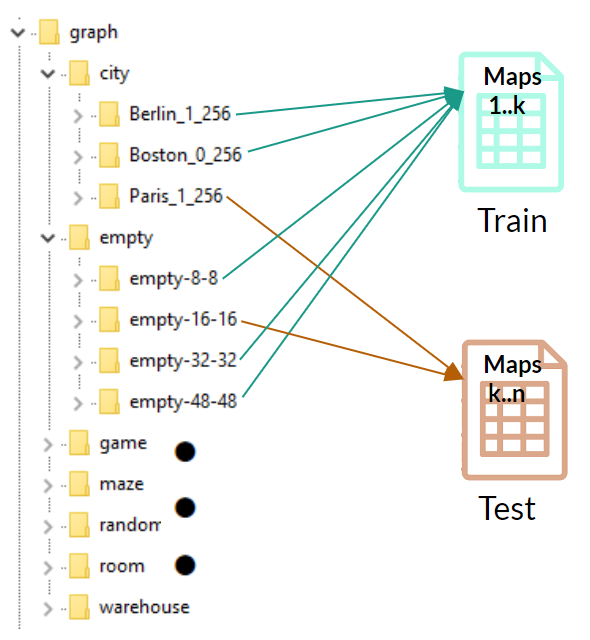
\includegraphics[scale=0.36]{Images/InGridTypeSetup.png}
%     \caption{In grid type split example}
%     \label{fig:InGridType}
% \end{figure}

% FEATHER algorithm requires all graphs cached for learning the their embeddings, thus due to this memory limitation for each experiment we used 5000 randomly selected samples from train set to train Graph embeddings  \Omri{What do you mean here?} \Carmel{I rephrased the sentence}
% MAPF samples were selected randomly within the constraint of “in grid type” setup.
% Only the “even” scenarios were used with all various sizes of number of agents.


%\subsection{MAPFGAS Experiment description} \vspace{10px}

% \subsubsection{\textbf{High Level Design}} \vspace{10px}
% \label{scn:MAPFGAS design}
% First Phase is to perform Structural abstraction for each MAPF problem. We cast a MAPF problem to its Graph representation and add special artificial links between each agent's start and goal nodes, then  using the FEATHER Algorithm presented in section \ref{scn:Feather}, we train it with all Graphs obtained from train set. By training this model we preform an unsupervised learning for the train MAPF problems Graph representations, The trained resulting model is used to get all graphs embeddings which is used later for training and testing a Machine Learning (ML) model.

% In the second phase we use the graphs embedding calculated from previous phase for each MAPF problem to train a verity of ML classification models. The dataset for classification models will be constructed for each MAPF problem vector as a concatenation between Graph Embedding and its special handcrafted features presented by Kaduri {\cite{kaduri2020algorithm}}.

% Figure \ref{fig:MAPFASG flow} illustrates how the structural abstractions combined to a sample used to train/test a classifier. 

% \begin{figure}[!h]
%     \centering
%     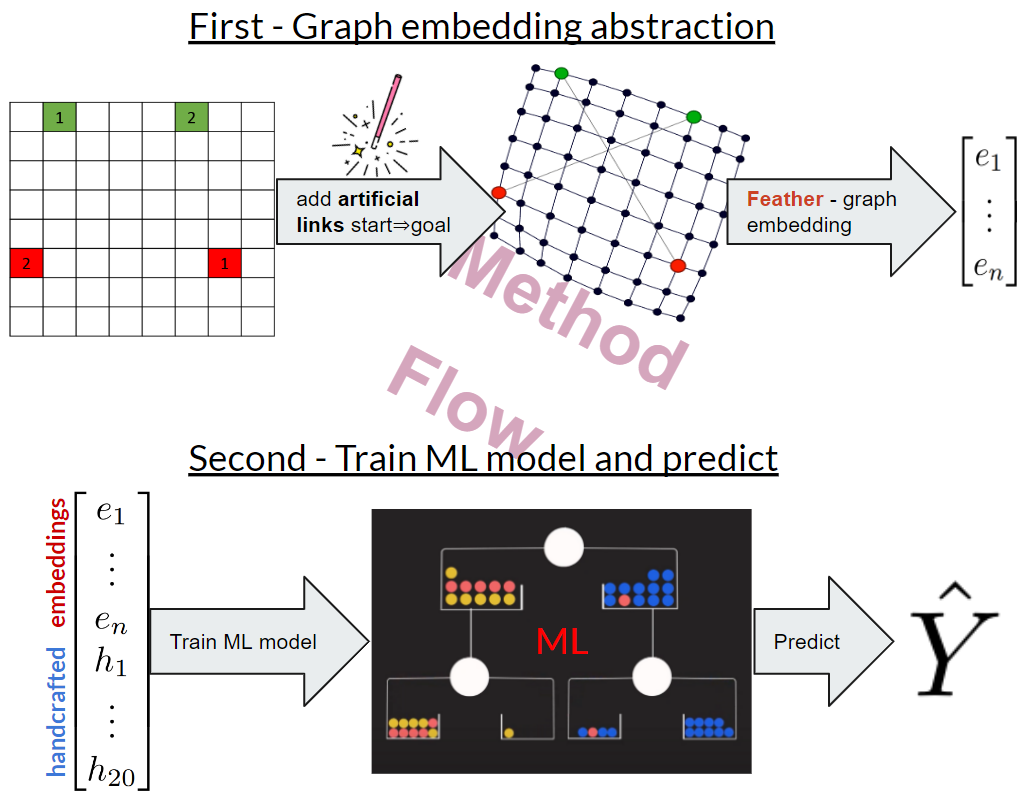
\includegraphics[scale=0.30]{Images/MAPFASG_flow.png}
%     \caption{High level design experiment of MAPFGAS}
%     \label{fig:MAPFASG flow}
% \end{figure}

% \subsubsection{\textbf{Structural Abstraction}} \vspace{10px}
% For structural abstraction shown we have used \href{https://github.com/benedekrozemberczki/karateclub/tree/master/karateclub/graph_embedding/}{Feather Graph embedding model} provided by the  Benedek et al. \cite{rozemberczki2020characteristic}, with the following non default hyper parameters: pooling='max'. The default value of 'pooling' is 'mean' resulting in much poor results, this is logical since node level features are pooled by the pooling method to create graph level statistics, and the only deference related to FullG2V abstractions between graphs obtained from the same grid MAPF problems is the special artificial links between agents location. Basically there is very little difference between graphs from same grid, by max pooling we emphasize the differences between graphs embeddings which works better for training a classification model. \Roni{Excellent explanation}

% \subsubsection{\textbf{Training ML models}} \vspace{10px}
% \label{scn:train_ml}
% FEATHER algorithm requires all graphs cached for learning their embeddings 
% \Roni{what about the graphs in the test set? do we need them to be known a-priori during training?} \Carmel{Answer - no need to know the test set, it will just take more time to infer one graph by another}, thus due to this memory limitation for each experiment we used 5000 randomly selected samples from train set to train Graph embeddings, note using 2500 randomly selected samples was resulting similar performance. for Kaduri's handcrafted feature abstraction method evaluation all train-set problems used. \Roni{We discovered this was not true, and the training is useless}

%%%%%%%%%%%%

% For each train-test split setup explained in section \ref{scn:split setup} we performed experiments within each setup's restrictions.
% For every experiment 3 standalone methods for MAPF problems abstraction where evaluated and another 4 for all possible combinations to classifying the fastest solving algorithm:
% % using XGBoost \cite{chen2016xgboost}(after trying other ML models like Random forest and Logistic Regression):
% \begin{itemize}
%     \item Kaduri's \cite{kaduri2020algorithm} handcrafted features representing MAPF problem's topology.
%     \item G2V \cite{ren2021mapfast} with Graphs embeddings obtained with FEATHER algorithm by Benedek et al. \cite{rozemberczki2020characteristic}
%     \Roni{Throughout the paper you write Benedek et al. but it seems to be Rozemberczki and Sarkar. Who is it? ~\shortcite{rozemberczki2020characteristic}} \Carmel{you right his full name is Benedek Rozemberczki}\Roni{Ok. We use only the last name}
%     \item Our novel FullG2V with Graphs embeddings obtained using FEATHER algorithm by Benedek et al. \cite{rozemberczki2020characteristic}
% \end{itemize}


% % \Carmel{TODO: fix this paragraph} In the experiments we run the 3 Machine Learning algorithms to see which one preform best in terms of Accuracy which is the metric used for this dataset in the literature. For each experiment 4-fold cross validation was used for training in order to find the best hyper-parameters for each algorithm. Grid search performed with the following hyper parameters was chosen in order to find the best configuration for each algorithm that maximizes classification Accuracy.

% XGBoost \cite{chen2016xgboost} ML model was used as the classifying Model after initial experiments preformed comparing between different ML classifiers such as: Logistic Regression classifier, Random Forest and XGBoost which was the winner.

% The metrics used for this dataset in the literature for evaluating between the 3 methods are:
% \begin{itemize}
%     \item Accuracy : classifying the fastest solving Algorithm.
%     \item Coverage :  portion of MAPF problems solved under a time limit of 5 minutes.
%     \item Run-Time (RT) : total run-time took all predicted solvers for all MAPF problems.\footnote{We considered cases where the selected MAPF solver could not solve the problem within our 5 minutes time limit as having a run-time of 5 minutes. The same has been done in prior work on MAPF AS~\cite{kaduri2020algorithm,ren2021mapfast}.}
% \end{itemize}
%  For each experiment a 4-fold cross validation was performed during training in order to find XGBoost's best hyper parameters for each methods. Finally we run the classifiers against the test set.

% % \begin{itemize}
% %     \item Logistic Regression : penalty - [l1, l2] ; C - [5.99e-03, 4.64e-02, 3.59e-01, 2.78e+00, 2.15e+01, 1.66e+02, 1.29e+03] ; solver - [lbfgs, liblinear]
% %     \item Random Forest : n\_estimators - [50, 60, 70, 80, 90, 100] ; max\_depth - [5, 6, 7, 8] ; criterion - [gini, entropy] ; max\_features -  [0.05, 0.1, 0.15, 0.2, 0.25]
% %     \item XGBoost : min\_child\_weight - [2, 3, 4, 5, 6, 7, 9, 10] ; gamma - [1.1, 1.2, 1.3] ; subsample - [0.95, 0.975, 1.0] ; colsample\_bytree -  [0.45, 0.5, 0.55] ; max\_depth - [5, 6] ; learning\_rate: [5e-06, 1e-05, 5e-05]
% % \end{itemize}


% % For each algorithm we selected the hyper-parameters that achieved the best Accuracy. With those parameters we train each of the classifiers using the whole training set. Finally we run the classifiers against the test set.

% % \textbf{Feature importance} analysis will be preformed using the best classifier achieved. 
% % we will use a feature selection method based on importance weights. finally we could assess what variables had little influence on prediction.


% \section{Results}
% \label{scn:RESULTS}

% Final resulting Table \ref{tab:prev_sota} represents the previous baseline results shown in paper \cite{ren2021mapfast} together with our best result achieved by MAPFGAS at "in grid split" setup. The table consists first from the result by Karuri's work \cite{kaduri2020algorithm} named 'XGBoost Cl', then new proposed method at the bottom of table called MAPFGAS.

% More information will be provided on MAPFGAS model performance in next section \ref{scn:MAPFASG result}
% \Roni{What's the ``Rerun'' column?} \Carmel{ its 'reproduced' by us}

% \begin{table}[!h]
%     \centering
% \begin{tabular}{ |c||c|c|c|c| }
% \hline
% \textbf{Method} & Acc  & Cov & Rerun & RT$_{minutes}$ \\ 
% %   min \# ending negatives &  \multicolumn{4}{|c|}{sliding window size} \\ 
%  \hline
  
% %  CNN$_{Class}$  & 0.7118  \\   

%   MAPFAST & 0.69 & 0.940 & F & \\ 
%   MAPFASTer & 0.75 & 0.956 & F & \\
%   % G2V & 0.71 & 0.95 & F & \\ 
%   G2V$_{rerun}$ & 0.81 & 0.968 & T & 10513 \\ 
%   XGBoost Cl &  0.83 & \textbf{0.979} & T & 9803 \\  

% % MAPFAST & 0.7689  & &\\  
%  FullG2v$_{alone}$ & 0.84 & \textbf{0.981} & NA & 9527\\
%   \textbf{MAPFGAS} & \textbf{0.85} & \textbf{0.986} & NA & \textbf{9180}\\  
%  \hline
 
% \end{tabular}
%     \caption{'In Grid Setup' baseline results with new methods  \Roni{How did we get the results for MAPFASTer? also, in ALL graphs please use 2 digits after the decimal points at most (for runtime no need for any digit beyond the decimal point.)} \Carmel{we got MAPFASTER result from paper you sent me}}
%     \label{tab:prev_sota}
% \end{table}

% % \begin{center}
% % \begin{tabular}{ |c|c|c|c| }
% % \hline
% % Method & Pre  & Rec   & f1  \\ 
% % %   min \# ending negatives &  \multicolumn{4}{|c|}{sliding window size} \\ 
% %  \hline
% %     & 100  & 250   & 500  \\  
% %  25  & x & x & x \\ 
% %  50 & x & x & x \\ 
% %  \hline
 
% % \end{tabular}
% % \label{tab:prev_sota}
% % \end{center}


% \subsection{MAPFGAS v.s. other method} \vspace{10px}
% \label{scn:MAPFASG result}




% Please add the following required packages to your document preamble:
% \usepackage{booktabs}
% \usepackage{multirow}
% \begin{table}
% \begin{tabular}{@{}llrrrrrrrrr@{}}
%                            & AS Setup & \multicolumn{3}{c}{In-Grid}                                                 & \multicolumn{3}{c}{In-Grid-Type}                                            & \multicolumn{3}{c}{Between-Grid}                                            \\
% Grid-type                  & Metric   & \multicolumn{1}{c}{KBS} & \multicolumn{1}{c}{G2V} & \multicolumn{1}{c}{MAG} & \multicolumn{1}{c}{KBS} & \multicolumn{1}{c}{G2V} & \multicolumn{1}{c}{MAG} & \multicolumn{1}{c}{KBS} & \multicolumn{1}{c}{G2V} & \multicolumn{1}{c}{MAG} \\
% \multirow{3}{*}{Empty}     & Acc      & 0.88                    & 0.89                    & 0.90                    & 0.67                    & 0.68                    & 0.71                    & 0.81                    & 0.78                    & 0.82                    \\
%                            & Cov      & 1.00                    & 1.00                    & 1.00                    & 0.97                    & 1.00                    & 0.99                    & 1.00                    & 0.99                    & 1.00                    \\
%                            & \%Rg     & 0.9                     & 0.1                     & 0.8                     & 3.5                     & 1.0                     & 1.8                     & 9.5                     & 17.7                    & 2.5                     \\
% \multirow{3}{*}{Random}    & Acc      & 0.91                    & 0.90                    & 0.91                    & 0.84                    & 0.79                    & 0.82                    & 0.78                    & 0.71                    & 0.73                    \\
%                            & Cov      & 1.00                    & 1.00                    & 1.00                    & 1.00                    & 0.99                    & 1.00                    & 1.00                    & 0.99                    & 1.00                    \\
%                            & \%Rg     & 3.1                     & 4.1                     & 2.4                     & 1.4                     & 2.3                     & 1.1                     & 7.2                     & 54.8                    & 4.0                     \\
% \multirow{3}{*}{Warehouse} & Acc      & 0.84                    & 0.84                    & 0.86                    & 0.64                    & 0.64                    & 0.67                    & 0.67                    & 0.62                    & 0.68                    \\
%                            & Cov      & 0.99                    & 0.99                    & 1.00                    & 0.94                    & 0.94                    & 0.96                    & 0.96                    & 0.88                    & 0.98                    \\
%                            & \%Rg     & 7.9                     & 9.4                     & 4.7                     & 1.4                     & 1.6                     & 1.3                     & 32.9                    & 78.1                    & 27.3                    \\
% \multirow{3}{*}{Game}      & Acc      & 0.91                    & 0.91                    & 0.92                    & 0.77                    & 0.72                    & 0.78                    & 0.74                    & 0.72                    & 0.65                    \\
%                            & Cov      & 0.98                    & 0.98                    & 0.99                    & 0.92                    & 0.86                    & 0.92                    & 0.88                    & 0.89                    & 0.89                    \\
%                            & \%Rg     & 19.2                    & 21.0                    & 18.0                    & 1.4                     & 2.3                     & 1.7                     & 122.0                   & 113.1                   & 122.0                   \\
% \multirow{3}{*}{City}      & Acc      & 0.90                    & 0.89                    & 0.92                    & 0.58                    & 0.57                    & 0.61                    & 0.53                    & 0.53                    & 0.58                    \\
%                            & Cov      & 0.99                    & 0.99                    & 0.99                    & 0.81                    & 0.83                    & 0.83                    & 0.90                    & 0.86                    & 0.88                    \\
%                            & \%Rg     & 10.1                    & 12.4                    & 7.1                     & 3.1                     & 3.0                     & 2.9                     & 136.2                   & 155.6                   & 146.3                   \\
% \multirow{3}{*}{Maze}      & Acc      & 0.85                    & 0.79                    & 0.86                    & 0.40                    & 0.44                    & 0.50                    & 0.56                    & 0.45                    & 0.47                    \\
%                            & Cov      & 0.98                    & 0.93                    & 0.99                    & 0.66                    & 0.62                    & 0.66                    & 0.71                    & 0.64                    & 0.66                    \\
%                            & \%Rg     & 31.9                    & 119.3                   & 20.6                    & 8.2                     & 9.6                     & 8.4                     & 398.8                   & 511.4                   & 483.6                   \\
% \multirow{3}{*}{Room}      & Acc      & 0.93                    & 0.90                    & 0.92                    & 0.63                    & 0.50                    & 0.66                    & 0.32                    & 0.43                    & 0.49                    \\
%                            & Cov      & 1.00                    & 1.00                    & 1.00                    & 0.91                    & 0.83                    & 0.94                    & 0.65                    & 0.75                    & 0.81                    \\
%                            & \%Rg     & 0.2                     & 2.1                     & 0.1                     & 2.9                     & 5.0                     & 2.2                     & 855.6                   & 614.5                   & 475.0                  
% \end{tabular}
% \end{table}
% % Please add the following required packages to your document preamble:
% % \usepackage{booktabs}
% % \usepackage{multirow}
% \begin{table}
% \begin{tabular}{@{}ll|rrr|rrr@{}}
% \toprule
%                            &        & \multicolumn{3}{c}{In-Grid} & \multicolumn{3}{c}{Between-Grid} \\ 
% Grid-type                  & Metric & KBS    & G2V     & MAG   & KBS       & G2V      & MAG    \\ \midrule
% \multirow{3}{*}{Empty}     & Acc    & 0.88   & 0.89    & \textbf{0.90}     & 0.81      & 0.78     & \textbf{0.82}      \\
%                            & Cov    & \textbf{1.00}   & \textbf{1.00}    & \textbf{1.00}     & \textbf{1.00}      & 0.99     & \textbf{1.00}      \\
%                            & \%Rg   & 0.9    & \textbf{0.1}     & 0.8      & 9.5       & 17.7     & \textbf{2.5}       \\\midrule
% \multirow{3}{*}{Random}    & Acc    & \textbf{0.91}   & 0.90    & \textbf{0.91}     & \textbf{0.78}      & 0.71     & 0.73      \\
%                            & Cov    & \textbf{1.00}   & \textbf{1.00}    & \textbf{1.00}     & \textbf{1.00}      & 0.99     & \textbf{1.00}      \\
%                            & \%Rg   & 3.1    & 4.1     & \textbf{2.4}      & 7.2       & 54.8     & \textbf{4.0}       \\\midrule
% \multirow{3}{*}{Warehouse} & Acc    & 0.84   & 0.84    & \textbf{0.86}     & 0.67      & 0.62     & \textbf{0.68}      \\
%                            & Cov    & 0.99   & 0.99    & \textbf{1.00}     & 0.96      & 0.88     & \textbf{0.98}      \\
%                            & \%Rg   & 7.9    & 9.4     & \textbf{4.7}      & 32.9      & 78.1     & \textbf{27.3}      \\ \midrule 
% \multirow{3}{*}{Game}      & Acc    & 0.91   & 0.91    & \textbf{0.92}     & \textbf{0.74}      & 0.72     & 0.65      \\
%                            & Cov    & 0.98   & 0.98    & \textbf{0.99}     & 0.88      & \textbf{0.89}     & \textbf{0.89}      \\
%                            & \%Rg   & 19.2   & 21.0    & \textbf{18.0}     & 122.0     & \textbf{113.1}    & 122.0     \\\midrule
% \multirow{3}{*}{City}      & Acc    & 0.90   & 0.89    & \textbf{0.92}     & 0.53      & 0.53     & \textbf{0.58}      \\
%                            & Cov    & \textbf{0.99}   & \textbf{0.99}    & \textbf{0.99}     & \textbf{0.90}      & 0.86     & 0.88      \\
%                            & \%Rg   & 10.1   & 12.4    & \textbf{7.1}      & \textbf{136.2}     & 155.6    & 146.3     \\\midrule
% \multirow{3}{*}{Maze}      & Acc    & 0.85   & 0.79    & \textbf{0.86}     & \textbf{0.56}      & 0.45     & 0.47      \\
%                            & Cov    & 0.98   & 0.93    & \textbf{0.99}     & \textbf{0.71}      & 0.64     & 0.66      \\
%                            & \%Rg   & 31.9   & 119.3   & \textbf{20.6}     & \textbf{398.8}     & 511.4    & 483.6     \\\midrule
% \multirow{3}{*}{Room}      & Acc    & \textbf{0.93}   & 0.90    & 0.92     & 0.32      & 0.43     & \textbf{0.49}      \\
%                            & Cov    & \textbf{1.00}   & \textbf{1.00}    & \textbf{1.00}     & 0.65      & 0.75     & \textbf{0.81}      \\
%                            & \%Rg   & 0.2    & 2.1     & \textbf{0.1}      & 855.6     & 614.5    & \textbf{475.0}     \\\bottomrule
% \end{tabular}
% \label{tab:by-grid-type}
% \caption{In-grid and between-grid-type results, grouped by test grid type.}
% \end{table}




% Please add the following required packages to your document preamble:
% \usepackage{booktabs}
% \usepackage{multirow}